% Created by tikzDevice version 0.10.1 on 2017-12-04 15:15:18
% !TEX encoding = UTF-8 Unicode
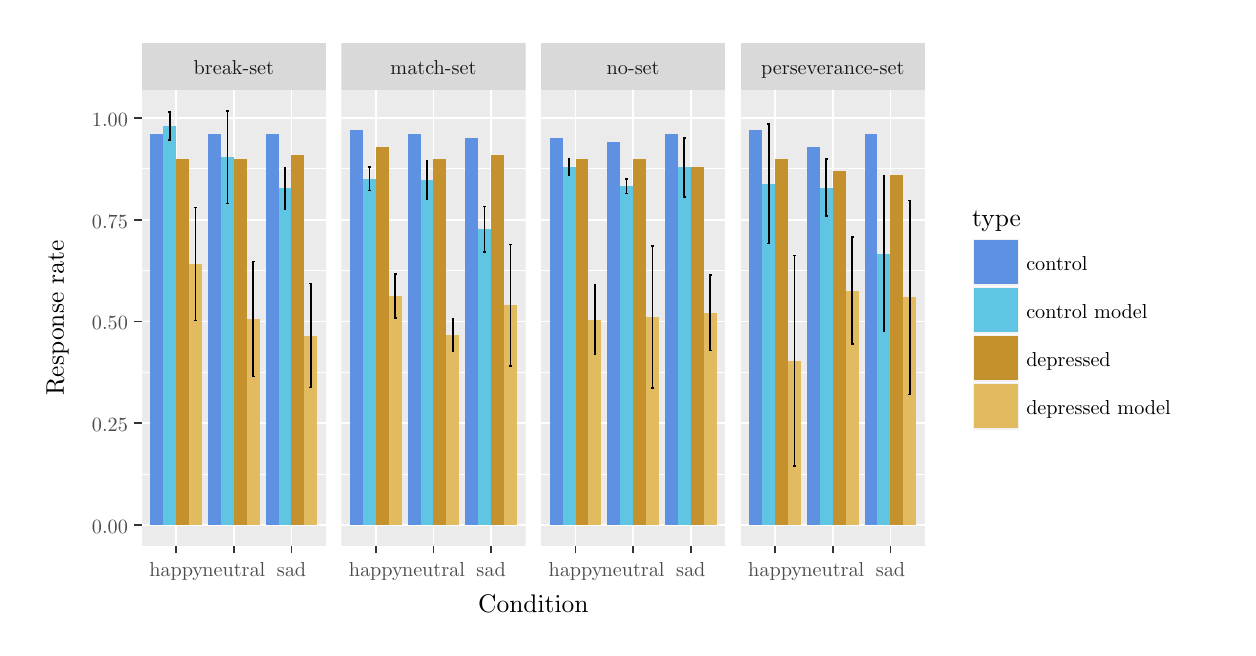
\begin{tikzpicture}[x=1pt,y=1pt]
\definecolor{fillColor}{RGB}{255,255,255}
\path[use as bounding box,fill=fillColor,fill opacity=0.00] (0,0) rectangle (433.62,216.81);
\begin{scope}
\path[clip] (  0.00,  0.00) rectangle (433.62,216.81);
\definecolor{drawColor}{RGB}{255,255,255}
\definecolor{fillColor}{RGB}{255,255,255}

\path[draw=drawColor,line width= 0.6pt,line join=round,line cap=round,fill=fillColor] (  0.00,  0.00) rectangle (433.62,216.81);
\end{scope}
\begin{scope}
\path[clip] ( 41.17, 29.59) rectangle (107.82,194.25);
\definecolor{fillColor}{gray}{0.92}

\path[fill=fillColor] ( 41.17, 29.59) rectangle (107.82,194.25);
\definecolor{drawColor}{RGB}{255,255,255}

\path[draw=drawColor,line width= 0.3pt,line join=round] ( 41.17, 55.46) --
	(107.82, 55.46);

\path[draw=drawColor,line width= 0.3pt,line join=round] ( 41.17, 92.23) --
	(107.82, 92.23);

\path[draw=drawColor,line width= 0.3pt,line join=round] ( 41.17,129.00) --
	(107.82,129.00);

\path[draw=drawColor,line width= 0.3pt,line join=round] ( 41.17,165.77) --
	(107.82,165.77);

\path[draw=drawColor,line width= 0.6pt,line join=round] ( 41.17, 37.07) --
	(107.82, 37.07);

\path[draw=drawColor,line width= 0.6pt,line join=round] ( 41.17, 73.84) --
	(107.82, 73.84);

\path[draw=drawColor,line width= 0.6pt,line join=round] ( 41.17,110.61) --
	(107.82,110.61);

\path[draw=drawColor,line width= 0.6pt,line join=round] ( 41.17,147.38) --
	(107.82,147.38);

\path[draw=drawColor,line width= 0.6pt,line join=round] ( 41.17,184.16) --
	(107.82,184.16);

\path[draw=drawColor,line width= 0.6pt,line join=round] ( 53.67, 29.59) --
	( 53.67,194.25);

\path[draw=drawColor,line width= 0.6pt,line join=round] ( 74.50, 29.59) --
	( 74.50,194.25);

\path[draw=drawColor,line width= 0.6pt,line join=round] ( 95.32, 29.59) --
	( 95.32,194.25);
\definecolor{fillColor}{RGB}{226,186,95}

\path[fill=fillColor] ( 58.36, 37.07) rectangle ( 63.04,131.44);
\definecolor{fillColor}{RGB}{196,145,45}

\path[fill=fillColor] ( 53.67, 37.07) rectangle ( 58.36,169.45);
\definecolor{fillColor}{RGB}{95,197,226}

\path[fill=fillColor] ( 48.98, 37.07) rectangle ( 53.67,181.27);
\definecolor{fillColor}{RGB}{95,145,226}

\path[fill=fillColor] ( 44.30, 37.07) rectangle ( 48.98,178.27);
\definecolor{fillColor}{RGB}{226,186,95}

\path[fill=fillColor] ( 79.18, 37.07) rectangle ( 83.87,111.49);
\definecolor{fillColor}{RGB}{196,145,45}

\path[fill=fillColor] ( 74.50, 37.07) rectangle ( 79.18,169.45);
\definecolor{fillColor}{RGB}{95,197,226}

\path[fill=fillColor] ( 69.81, 37.07) rectangle ( 74.50,169.99);
\definecolor{fillColor}{RGB}{95,145,226}

\path[fill=fillColor] ( 65.12, 37.07) rectangle ( 69.81,178.27);
\definecolor{fillColor}{RGB}{226,186,95}

\path[fill=fillColor] (100.01, 37.07) rectangle (104.69,105.56);
\definecolor{fillColor}{RGB}{196,145,45}

\path[fill=fillColor] ( 95.32, 37.07) rectangle (100.01,170.92);
\definecolor{fillColor}{RGB}{95,197,226}

\path[fill=fillColor] ( 90.64, 37.07) rectangle ( 95.32,158.76);
\definecolor{fillColor}{RGB}{95,145,226}

\path[fill=fillColor] ( 85.95, 37.07) rectangle ( 90.64,178.27);
\definecolor{drawColor}{RGB}{0,0,0}

\path[draw=drawColor,line width= 0.6pt,line join=round] ( 60.18,151.88) --
	( 61.22,151.88);

\path[draw=drawColor,line width= 0.6pt,line join=round] ( 60.70,151.88) --
	( 60.70,111.00);

\path[draw=drawColor,line width= 0.6pt,line join=round] ( 60.18,111.00) --
	( 61.22,111.00);

\path[draw=drawColor,line width= 0.6pt,line join=round] ( 50.81,186.27) --
	( 51.85,186.27);

\path[draw=drawColor,line width= 0.6pt,line join=round] ( 51.33,186.27) --
	( 51.33,176.28);

\path[draw=drawColor,line width= 0.6pt,line join=round] ( 50.81,176.28) --
	( 51.85,176.28);

\path[draw=drawColor,line width= 0.6pt,line join=round] ( 81.00,132.28) --
	( 82.05,132.28);

\path[draw=drawColor,line width= 0.6pt,line join=round] ( 81.52,132.28) --
	( 81.52, 90.70);

\path[draw=drawColor,line width= 0.6pt,line join=round] ( 81.00, 90.70) --
	( 82.05, 90.70);

\path[draw=drawColor,line width= 0.6pt,line join=round] ( 71.63,186.76) --
	( 72.67,186.76);

\path[draw=drawColor,line width= 0.6pt,line join=round] ( 72.15,186.76) --
	( 72.15,153.22);

\path[draw=drawColor,line width= 0.6pt,line join=round] ( 71.63,153.22) --
	( 72.67,153.22);

\path[draw=drawColor,line width= 0.6pt,line join=round] (101.83,124.37) --
	(102.87,124.37);

\path[draw=drawColor,line width= 0.6pt,line join=round] (102.35,124.37) --
	(102.35, 86.76);

\path[draw=drawColor,line width= 0.6pt,line join=round] (101.83, 86.76) --
	(102.87, 86.76);

\path[draw=drawColor,line width= 0.6pt,line join=round] ( 92.46,166.32) --
	( 93.50,166.32);

\path[draw=drawColor,line width= 0.6pt,line join=round] ( 92.98,166.32) --
	( 92.98,151.21);

\path[draw=drawColor,line width= 0.6pt,line join=round] ( 92.46,151.21) --
	( 93.50,151.21);
\end{scope}
\begin{scope}
\path[clip] (113.32, 29.59) rectangle (179.96,194.25);
\definecolor{fillColor}{gray}{0.92}

\path[fill=fillColor] (113.32, 29.59) rectangle (179.96,194.25);
\definecolor{drawColor}{RGB}{255,255,255}

\path[draw=drawColor,line width= 0.3pt,line join=round] (113.32, 55.46) --
	(179.96, 55.46);

\path[draw=drawColor,line width= 0.3pt,line join=round] (113.32, 92.23) --
	(179.96, 92.23);

\path[draw=drawColor,line width= 0.3pt,line join=round] (113.32,129.00) --
	(179.96,129.00);

\path[draw=drawColor,line width= 0.3pt,line join=round] (113.32,165.77) --
	(179.96,165.77);

\path[draw=drawColor,line width= 0.6pt,line join=round] (113.32, 37.07) --
	(179.96, 37.07);

\path[draw=drawColor,line width= 0.6pt,line join=round] (113.32, 73.84) --
	(179.96, 73.84);

\path[draw=drawColor,line width= 0.6pt,line join=round] (113.32,110.61) --
	(179.96,110.61);

\path[draw=drawColor,line width= 0.6pt,line join=round] (113.32,147.38) --
	(179.96,147.38);

\path[draw=drawColor,line width= 0.6pt,line join=round] (113.32,184.16) --
	(179.96,184.16);

\path[draw=drawColor,line width= 0.6pt,line join=round] (125.81, 29.59) --
	(125.81,194.25);

\path[draw=drawColor,line width= 0.6pt,line join=round] (146.64, 29.59) --
	(146.64,194.25);

\path[draw=drawColor,line width= 0.6pt,line join=round] (167.47, 29.59) --
	(167.47,194.25);
\definecolor{fillColor}{RGB}{226,186,95}

\path[fill=fillColor] (130.50, 37.07) rectangle (135.19,119.86);
\definecolor{fillColor}{RGB}{196,145,45}

\path[fill=fillColor] (125.81, 37.07) rectangle (130.50,173.86);
\definecolor{fillColor}{RGB}{95,197,226}

\path[fill=fillColor] (121.13, 37.07) rectangle (125.81,162.26);
\definecolor{fillColor}{RGB}{95,145,226}

\path[fill=fillColor] (116.44, 37.07) rectangle (121.13,179.74);
\definecolor{fillColor}{RGB}{226,186,95}

\path[fill=fillColor] (151.33, 37.07) rectangle (156.01,105.77);
\definecolor{fillColor}{RGB}{196,145,45}

\path[fill=fillColor] (146.64, 37.07) rectangle (151.33,169.45);
\definecolor{fillColor}{RGB}{95,197,226}

\path[fill=fillColor] (141.95, 37.07) rectangle (146.64,161.63);
\definecolor{fillColor}{RGB}{95,145,226}

\path[fill=fillColor] (137.27, 37.07) rectangle (141.95,178.27);
\definecolor{fillColor}{RGB}{226,186,95}

\path[fill=fillColor] (172.15, 37.07) rectangle (176.84,116.48);
\definecolor{fillColor}{RGB}{196,145,45}

\path[fill=fillColor] (167.47, 37.07) rectangle (172.15,170.92);
\definecolor{fillColor}{RGB}{95,197,226}

\path[fill=fillColor] (162.78, 37.07) rectangle (167.47,143.94);
\definecolor{fillColor}{RGB}{95,145,226}

\path[fill=fillColor] (158.10, 37.07) rectangle (162.78,176.80);
\definecolor{drawColor}{RGB}{0,0,0}

\path[draw=drawColor,line width= 0.6pt,line join=round] (132.32,127.86) --
	(133.36,127.86);

\path[draw=drawColor,line width= 0.6pt,line join=round] (132.84,127.86) --
	(132.84,111.86);

\path[draw=drawColor,line width= 0.6pt,line join=round] (132.32,111.86) --
	(133.36,111.86);

\path[draw=drawColor,line width= 0.6pt,line join=round] (122.95,166.53) --
	(123.99,166.53);

\path[draw=drawColor,line width= 0.6pt,line join=round] (123.47,166.53) --
	(123.47,158.00);

\path[draw=drawColor,line width= 0.6pt,line join=round] (122.95,158.00) --
	(123.99,158.00);

\path[draw=drawColor,line width= 0.6pt,line join=round] (153.15,111.57) --
	(154.19,111.57);

\path[draw=drawColor,line width= 0.6pt,line join=round] (153.67,111.57) --
	(153.67, 99.97);

\path[draw=drawColor,line width= 0.6pt,line join=round] (153.15, 99.97) --
	(154.19, 99.97);

\path[draw=drawColor,line width= 0.6pt,line join=round] (143.78,168.54) --
	(144.82,168.54);

\path[draw=drawColor,line width= 0.6pt,line join=round] (144.30,168.54) --
	(144.30,154.72);

\path[draw=drawColor,line width= 0.6pt,line join=round] (143.78,154.72) --
	(144.82,154.72);

\path[draw=drawColor,line width= 0.6pt,line join=round] (173.98,138.48) --
	(175.02,138.48);

\path[draw=drawColor,line width= 0.6pt,line join=round] (174.50,138.48) --
	(174.50, 94.47);

\path[draw=drawColor,line width= 0.6pt,line join=round] (173.98, 94.47) --
	(175.02, 94.47);

\path[draw=drawColor,line width= 0.6pt,line join=round] (164.60,152.19) --
	(165.64,152.19);

\path[draw=drawColor,line width= 0.6pt,line join=round] (165.12,152.19) --
	(165.12,135.69);

\path[draw=drawColor,line width= 0.6pt,line join=round] (164.60,135.69) --
	(165.64,135.69);
\end{scope}
\begin{scope}
\path[clip] (185.46, 29.59) rectangle (252.11,194.25);
\definecolor{fillColor}{gray}{0.92}

\path[fill=fillColor] (185.46, 29.59) rectangle (252.11,194.25);
\definecolor{drawColor}{RGB}{255,255,255}

\path[draw=drawColor,line width= 0.3pt,line join=round] (185.46, 55.46) --
	(252.11, 55.46);

\path[draw=drawColor,line width= 0.3pt,line join=round] (185.46, 92.23) --
	(252.11, 92.23);

\path[draw=drawColor,line width= 0.3pt,line join=round] (185.46,129.00) --
	(252.11,129.00);

\path[draw=drawColor,line width= 0.3pt,line join=round] (185.46,165.77) --
	(252.11,165.77);

\path[draw=drawColor,line width= 0.6pt,line join=round] (185.46, 37.07) --
	(252.11, 37.07);

\path[draw=drawColor,line width= 0.6pt,line join=round] (185.46, 73.84) --
	(252.11, 73.84);

\path[draw=drawColor,line width= 0.6pt,line join=round] (185.46,110.61) --
	(252.11,110.61);

\path[draw=drawColor,line width= 0.6pt,line join=round] (185.46,147.38) --
	(252.11,147.38);

\path[draw=drawColor,line width= 0.6pt,line join=round] (185.46,184.16) --
	(252.11,184.16);

\path[draw=drawColor,line width= 0.6pt,line join=round] (197.96, 29.59) --
	(197.96,194.25);

\path[draw=drawColor,line width= 0.6pt,line join=round] (218.79, 29.59) --
	(218.79,194.25);

\path[draw=drawColor,line width= 0.6pt,line join=round] (239.61, 29.59) --
	(239.61,194.25);
\definecolor{fillColor}{RGB}{226,186,95}

\path[fill=fillColor] (202.64, 37.07) rectangle (207.33,111.28);
\definecolor{fillColor}{RGB}{196,145,45}

\path[fill=fillColor] (197.96, 37.07) rectangle (202.64,169.45);
\definecolor{fillColor}{RGB}{95,197,226}

\path[fill=fillColor] (193.27, 37.07) rectangle (197.96,166.38);
\definecolor{fillColor}{RGB}{95,145,226}

\path[fill=fillColor] (188.59, 37.07) rectangle (193.27,176.80);
\definecolor{fillColor}{RGB}{226,186,95}

\path[fill=fillColor] (223.47, 37.07) rectangle (228.16,112.28);
\definecolor{fillColor}{RGB}{196,145,45}

\path[fill=fillColor] (218.79, 37.07) rectangle (223.47,169.45);
\definecolor{fillColor}{RGB}{95,197,226}

\path[fill=fillColor] (214.10, 37.07) rectangle (218.79,159.44);
\definecolor{fillColor}{RGB}{95,145,226}

\path[fill=fillColor] (209.41, 37.07) rectangle (214.10,175.33);
\definecolor{fillColor}{RGB}{226,186,95}

\path[fill=fillColor] (244.30, 37.07) rectangle (248.98,113.77);
\definecolor{fillColor}{RGB}{196,145,45}

\path[fill=fillColor] (239.61, 37.07) rectangle (244.30,166.51);
\definecolor{fillColor}{RGB}{95,197,226}

\path[fill=fillColor] (234.93, 37.07) rectangle (239.61,166.33);
\definecolor{fillColor}{RGB}{95,145,226}

\path[fill=fillColor] (230.24, 37.07) rectangle (234.93,178.27);
\definecolor{drawColor}{RGB}{0,0,0}

\path[draw=drawColor,line width= 0.6pt,line join=round] (204.47,123.81) --
	(205.51,123.81);

\path[draw=drawColor,line width= 0.6pt,line join=round] (204.99,123.81) --
	(204.99, 98.76);

\path[draw=drawColor,line width= 0.6pt,line join=round] (204.47, 98.76) --
	(205.51, 98.76);

\path[draw=drawColor,line width= 0.6pt,line join=round] (195.10,169.41) --
	(196.14,169.41);

\path[draw=drawColor,line width= 0.6pt,line join=round] (195.62,169.41) --
	(195.62,163.35);

\path[draw=drawColor,line width= 0.6pt,line join=round] (195.10,163.35) --
	(196.14,163.35);

\path[draw=drawColor,line width= 0.6pt,line join=round] (225.29,137.87) --
	(226.34,137.87);

\path[draw=drawColor,line width= 0.6pt,line join=round] (225.81,137.87) --
	(225.81, 86.69);

\path[draw=drawColor,line width= 0.6pt,line join=round] (225.29, 86.69) --
	(226.34, 86.69);

\path[draw=drawColor,line width= 0.6pt,line join=round] (215.92,162.04) --
	(216.96,162.04);

\path[draw=drawColor,line width= 0.6pt,line join=round] (216.44,162.04) --
	(216.44,156.85);

\path[draw=drawColor,line width= 0.6pt,line join=round] (215.92,156.85) --
	(216.96,156.85);

\path[draw=drawColor,line width= 0.6pt,line join=round] (246.12,127.41) --
	(247.16,127.41);

\path[draw=drawColor,line width= 0.6pt,line join=round] (246.64,127.41) --
	(246.64,100.13);

\path[draw=drawColor,line width= 0.6pt,line join=round] (246.12,100.13) --
	(247.16,100.13);

\path[draw=drawColor,line width= 0.6pt,line join=round] (236.75,176.93) --
	(237.79,176.93);

\path[draw=drawColor,line width= 0.6pt,line join=round] (237.27,176.93) --
	(237.27,155.73);

\path[draw=drawColor,line width= 0.6pt,line join=round] (236.75,155.73) --
	(237.79,155.73);
\end{scope}
\begin{scope}
\path[clip] (257.61, 29.59) rectangle (324.25,194.25);
\definecolor{fillColor}{gray}{0.92}

\path[fill=fillColor] (257.61, 29.59) rectangle (324.25,194.25);
\definecolor{drawColor}{RGB}{255,255,255}

\path[draw=drawColor,line width= 0.3pt,line join=round] (257.61, 55.46) --
	(324.25, 55.46);

\path[draw=drawColor,line width= 0.3pt,line join=round] (257.61, 92.23) --
	(324.25, 92.23);

\path[draw=drawColor,line width= 0.3pt,line join=round] (257.61,129.00) --
	(324.25,129.00);

\path[draw=drawColor,line width= 0.3pt,line join=round] (257.61,165.77) --
	(324.25,165.77);

\path[draw=drawColor,line width= 0.6pt,line join=round] (257.61, 37.07) --
	(324.25, 37.07);

\path[draw=drawColor,line width= 0.6pt,line join=round] (257.61, 73.84) --
	(324.25, 73.84);

\path[draw=drawColor,line width= 0.6pt,line join=round] (257.61,110.61) --
	(324.25,110.61);

\path[draw=drawColor,line width= 0.6pt,line join=round] (257.61,147.38) --
	(324.25,147.38);

\path[draw=drawColor,line width= 0.6pt,line join=round] (257.61,184.16) --
	(324.25,184.16);

\path[draw=drawColor,line width= 0.6pt,line join=round] (270.10, 29.59) --
	(270.10,194.25);

\path[draw=drawColor,line width= 0.6pt,line join=round] (290.93, 29.59) --
	(290.93,194.25);

\path[draw=drawColor,line width= 0.6pt,line join=round] (311.76, 29.59) --
	(311.76,194.25);
\definecolor{fillColor}{RGB}{226,186,95}

\path[fill=fillColor] (274.79, 37.07) rectangle (279.48, 96.45);
\definecolor{fillColor}{RGB}{196,145,45}

\path[fill=fillColor] (270.10, 37.07) rectangle (274.79,169.45);
\definecolor{fillColor}{RGB}{95,197,226}

\path[fill=fillColor] (265.42, 37.07) rectangle (270.10,160.34);
\definecolor{fillColor}{RGB}{95,145,226}

\path[fill=fillColor] (260.73, 37.07) rectangle (265.42,179.74);
\definecolor{fillColor}{RGB}{226,186,95}

\path[fill=fillColor] (295.62, 37.07) rectangle (300.30,121.76);
\definecolor{fillColor}{RGB}{196,145,45}

\path[fill=fillColor] (290.93, 37.07) rectangle (295.62,165.03);
\definecolor{fillColor}{RGB}{95,197,226}

\path[fill=fillColor] (286.24, 37.07) rectangle (290.93,159.00);
\definecolor{fillColor}{RGB}{95,145,226}

\path[fill=fillColor] (281.56, 37.07) rectangle (286.24,173.86);
\definecolor{fillColor}{RGB}{226,186,95}

\path[fill=fillColor] (316.44, 37.07) rectangle (321.13,119.33);
\definecolor{fillColor}{RGB}{196,145,45}

\path[fill=fillColor] (311.76, 37.07) rectangle (316.44,163.56);
\definecolor{fillColor}{RGB}{95,197,226}

\path[fill=fillColor] (307.07, 37.07) rectangle (311.76,135.13);
\definecolor{fillColor}{RGB}{95,145,226}

\path[fill=fillColor] (302.39, 37.07) rectangle (307.07,178.27);
\definecolor{drawColor}{RGB}{0,0,0}

\path[draw=drawColor,line width= 0.6pt,line join=round] (276.61,134.44) --
	(277.65,134.44);

\path[draw=drawColor,line width= 0.6pt,line join=round] (277.13,134.44) --
	(277.13, 58.46);

\path[draw=drawColor,line width= 0.6pt,line join=round] (276.61, 58.46) --
	(277.65, 58.46);

\path[draw=drawColor,line width= 0.6pt,line join=round] (267.24,181.91) --
	(268.28,181.91);

\path[draw=drawColor,line width= 0.6pt,line join=round] (267.76,181.91) --
	(267.76,138.78);

\path[draw=drawColor,line width= 0.6pt,line join=round] (267.24,138.78) --
	(268.28,138.78);

\path[draw=drawColor,line width= 0.6pt,line join=round] (297.44,141.06) --
	(298.48,141.06);

\path[draw=drawColor,line width= 0.6pt,line join=round] (297.96,141.06) --
	(297.96,102.46);

\path[draw=drawColor,line width= 0.6pt,line join=round] (297.44,102.46) --
	(298.48,102.46);

\path[draw=drawColor,line width= 0.6pt,line join=round] (288.07,169.34) --
	(289.11,169.34);

\path[draw=drawColor,line width= 0.6pt,line join=round] (288.59,169.34) --
	(288.59,148.66);

\path[draw=drawColor,line width= 0.6pt,line join=round] (288.07,148.66) --
	(289.11,148.66);

\path[draw=drawColor,line width= 0.6pt,line join=round] (318.27,154.39) --
	(319.31,154.39);

\path[draw=drawColor,line width= 0.6pt,line join=round] (318.79,154.39) --
	(318.79, 84.27);

\path[draw=drawColor,line width= 0.6pt,line join=round] (318.27, 84.27) --
	(319.31, 84.27);

\path[draw=drawColor,line width= 0.6pt,line join=round] (308.89,163.21) --
	(309.93,163.21);

\path[draw=drawColor,line width= 0.6pt,line join=round] (309.41,163.21) --
	(309.41,107.04);

\path[draw=drawColor,line width= 0.6pt,line join=round] (308.89,107.04) --
	(309.93,107.04);
\end{scope}
\begin{scope}
\path[clip] ( 41.17,194.25) rectangle (107.82,211.31);
\definecolor{fillColor}{gray}{0.85}

\path[fill=fillColor] ( 41.17,194.25) rectangle (107.82,211.31);
\definecolor{drawColor}{gray}{0.10}

\node[text=drawColor,anchor=base,inner sep=0pt, outer sep=0pt, scale=  0.73] at ( 74.50,199.75) {break-set};
\end{scope}
\begin{scope}
\path[clip] (113.32,194.25) rectangle (179.96,211.31);
\definecolor{fillColor}{gray}{0.85}

\path[fill=fillColor] (113.32,194.25) rectangle (179.96,211.31);
\definecolor{drawColor}{gray}{0.10}

\node[text=drawColor,anchor=base,inner sep=0pt, outer sep=0pt, scale=  0.73] at (146.64,199.75) {match-set};
\end{scope}
\begin{scope}
\path[clip] (185.46,194.25) rectangle (252.11,211.31);
\definecolor{fillColor}{gray}{0.85}

\path[fill=fillColor] (185.46,194.25) rectangle (252.11,211.31);
\definecolor{drawColor}{gray}{0.10}

\node[text=drawColor,anchor=base,inner sep=0pt, outer sep=0pt, scale=  0.73] at (218.79,199.75) {no-set};
\end{scope}
\begin{scope}
\path[clip] (257.61,194.25) rectangle (324.25,211.31);
\definecolor{fillColor}{gray}{0.85}

\path[fill=fillColor] (257.61,194.25) rectangle (324.25,211.31);
\definecolor{drawColor}{gray}{0.10}

\node[text=drawColor,anchor=base,inner sep=0pt, outer sep=0pt, scale=  0.73] at (290.93,199.75) {perseverance-set};
\end{scope}
\begin{scope}
\path[clip] (  0.00,  0.00) rectangle (433.62,216.81);
\definecolor{drawColor}{gray}{0.20}

\path[draw=drawColor,line width= 0.6pt,line join=round] ( 53.67, 26.84) --
	( 53.67, 29.59);

\path[draw=drawColor,line width= 0.6pt,line join=round] ( 74.50, 26.84) --
	( 74.50, 29.59);

\path[draw=drawColor,line width= 0.6pt,line join=round] ( 95.32, 26.84) --
	( 95.32, 29.59);
\end{scope}
\begin{scope}
\path[clip] (  0.00,  0.00) rectangle (433.62,216.81);
\definecolor{drawColor}{gray}{0.30}

\node[text=drawColor,anchor=base,inner sep=0pt, outer sep=0pt, scale=  0.73] at ( 53.67, 18.58) {happy};

\node[text=drawColor,anchor=base,inner sep=0pt, outer sep=0pt, scale=  0.73] at ( 74.50, 18.58) {neutral};

\node[text=drawColor,anchor=base,inner sep=0pt, outer sep=0pt, scale=  0.73] at ( 95.32, 18.58) {sad};
\end{scope}
\begin{scope}
\path[clip] (  0.00,  0.00) rectangle (433.62,216.81);
\definecolor{drawColor}{gray}{0.20}

\path[draw=drawColor,line width= 0.6pt,line join=round] (125.81, 26.84) --
	(125.81, 29.59);

\path[draw=drawColor,line width= 0.6pt,line join=round] (146.64, 26.84) --
	(146.64, 29.59);

\path[draw=drawColor,line width= 0.6pt,line join=round] (167.47, 26.84) --
	(167.47, 29.59);
\end{scope}
\begin{scope}
\path[clip] (  0.00,  0.00) rectangle (433.62,216.81);
\definecolor{drawColor}{gray}{0.30}

\node[text=drawColor,anchor=base,inner sep=0pt, outer sep=0pt, scale=  0.73] at (125.81, 18.58) {happy};

\node[text=drawColor,anchor=base,inner sep=0pt, outer sep=0pt, scale=  0.73] at (146.64, 18.58) {neutral};

\node[text=drawColor,anchor=base,inner sep=0pt, outer sep=0pt, scale=  0.73] at (167.47, 18.58) {sad};
\end{scope}
\begin{scope}
\path[clip] (  0.00,  0.00) rectangle (433.62,216.81);
\definecolor{drawColor}{gray}{0.20}

\path[draw=drawColor,line width= 0.6pt,line join=round] (197.96, 26.84) --
	(197.96, 29.59);

\path[draw=drawColor,line width= 0.6pt,line join=round] (218.79, 26.84) --
	(218.79, 29.59);

\path[draw=drawColor,line width= 0.6pt,line join=round] (239.61, 26.84) --
	(239.61, 29.59);
\end{scope}
\begin{scope}
\path[clip] (  0.00,  0.00) rectangle (433.62,216.81);
\definecolor{drawColor}{gray}{0.30}

\node[text=drawColor,anchor=base,inner sep=0pt, outer sep=0pt, scale=  0.73] at (197.96, 18.58) {happy};

\node[text=drawColor,anchor=base,inner sep=0pt, outer sep=0pt, scale=  0.73] at (218.79, 18.58) {neutral};

\node[text=drawColor,anchor=base,inner sep=0pt, outer sep=0pt, scale=  0.73] at (239.61, 18.58) {sad};
\end{scope}
\begin{scope}
\path[clip] (  0.00,  0.00) rectangle (433.62,216.81);
\definecolor{drawColor}{gray}{0.20}

\path[draw=drawColor,line width= 0.6pt,line join=round] (270.10, 26.84) --
	(270.10, 29.59);

\path[draw=drawColor,line width= 0.6pt,line join=round] (290.93, 26.84) --
	(290.93, 29.59);

\path[draw=drawColor,line width= 0.6pt,line join=round] (311.76, 26.84) --
	(311.76, 29.59);
\end{scope}
\begin{scope}
\path[clip] (  0.00,  0.00) rectangle (433.62,216.81);
\definecolor{drawColor}{gray}{0.30}

\node[text=drawColor,anchor=base,inner sep=0pt, outer sep=0pt, scale=  0.73] at (270.10, 18.58) {happy};

\node[text=drawColor,anchor=base,inner sep=0pt, outer sep=0pt, scale=  0.73] at (290.93, 18.58) {neutral};

\node[text=drawColor,anchor=base,inner sep=0pt, outer sep=0pt, scale=  0.73] at (311.76, 18.58) {sad};
\end{scope}
\begin{scope}
\path[clip] (  0.00,  0.00) rectangle (433.62,216.81);
\definecolor{drawColor}{gray}{0.30}

\node[text=drawColor,anchor=base east,inner sep=0pt, outer sep=0pt, scale=  0.73] at ( 36.22, 34.04) {0.00};

\node[text=drawColor,anchor=base east,inner sep=0pt, outer sep=0pt, scale=  0.73] at ( 36.22, 70.81) {0.25};

\node[text=drawColor,anchor=base east,inner sep=0pt, outer sep=0pt, scale=  0.73] at ( 36.22,107.58) {0.50};

\node[text=drawColor,anchor=base east,inner sep=0pt, outer sep=0pt, scale=  0.73] at ( 36.22,144.35) {0.75};

\node[text=drawColor,anchor=base east,inner sep=0pt, outer sep=0pt, scale=  0.73] at ( 36.22,181.13) {1.00};
\end{scope}
\begin{scope}
\path[clip] (  0.00,  0.00) rectangle (433.62,216.81);
\definecolor{drawColor}{gray}{0.20}

\path[draw=drawColor,line width= 0.6pt,line join=round] ( 38.42, 37.07) --
	( 41.17, 37.07);

\path[draw=drawColor,line width= 0.6pt,line join=round] ( 38.42, 73.84) --
	( 41.17, 73.84);

\path[draw=drawColor,line width= 0.6pt,line join=round] ( 38.42,110.61) --
	( 41.17,110.61);

\path[draw=drawColor,line width= 0.6pt,line join=round] ( 38.42,147.38) --
	( 41.17,147.38);

\path[draw=drawColor,line width= 0.6pt,line join=round] ( 38.42,184.16) --
	( 41.17,184.16);
\end{scope}
\begin{scope}
\path[clip] (  0.00,  0.00) rectangle (433.62,216.81);
\definecolor{drawColor}{RGB}{0,0,0}

\node[text=drawColor,anchor=base,inner sep=0pt, outer sep=0pt, scale=  0.92] at (182.71,  5.50) {Condition};
\end{scope}
\begin{scope}
\path[clip] (  0.00,  0.00) rectangle (433.62,216.81);
\definecolor{drawColor}{RGB}{0,0,0}

\node[text=drawColor,rotate= 90.00,anchor=base,inner sep=0pt, outer sep=0pt, scale=  0.92] at ( 13.08,111.92) {Response rate};
\end{scope}
\begin{scope}
\path[clip] (  0.00,  0.00) rectangle (433.62,216.81);
\definecolor{fillColor}{RGB}{255,255,255}

\path[fill=fillColor] (335.63, 65.58) rectangle (428.12,158.25);
\end{scope}
\begin{scope}
\path[clip] (  0.00,  0.00) rectangle (433.62,216.81);
\definecolor{drawColor}{RGB}{0,0,0}

\node[text=drawColor,anchor=base west,inner sep=0pt, outer sep=0pt, scale=  0.92] at (341.32,144.99) {type};
\end{scope}
\begin{scope}
\path[clip] (  0.00,  0.00) rectangle (433.62,216.81);
\definecolor{drawColor}{RGB}{255,255,255}
\definecolor{fillColor}{gray}{0.95}

\path[draw=drawColor,line width= 0.6pt,line join=round,line cap=round,fill=fillColor] (341.32,123.31) rectangle (358.67,140.65);
\end{scope}
\begin{scope}
\path[clip] (  0.00,  0.00) rectangle (433.62,216.81);
\definecolor{fillColor}{RGB}{95,145,226}

\path[fill=fillColor] (342.04,124.02) rectangle (357.96,139.94);
\end{scope}
\begin{scope}
\path[clip] (  0.00,  0.00) rectangle (433.62,216.81);
\definecolor{drawColor}{RGB}{255,255,255}
\definecolor{fillColor}{gray}{0.95}

\path[draw=drawColor,line width= 0.6pt,line join=round,line cap=round,fill=fillColor] (341.32,105.96) rectangle (358.67,123.31);
\end{scope}
\begin{scope}
\path[clip] (  0.00,  0.00) rectangle (433.62,216.81);
\definecolor{fillColor}{RGB}{95,197,226}

\path[fill=fillColor] (342.04,106.67) rectangle (357.96,122.60);
\end{scope}
\begin{scope}
\path[clip] (  0.00,  0.00) rectangle (433.62,216.81);
\definecolor{drawColor}{RGB}{255,255,255}
\definecolor{fillColor}{gray}{0.95}

\path[draw=drawColor,line width= 0.6pt,line join=round,line cap=round,fill=fillColor] (341.32, 88.62) rectangle (358.67,105.96);
\end{scope}
\begin{scope}
\path[clip] (  0.00,  0.00) rectangle (433.62,216.81);
\definecolor{fillColor}{RGB}{196,145,45}

\path[fill=fillColor] (342.04, 89.33) rectangle (357.96,105.25);
\end{scope}
\begin{scope}
\path[clip] (  0.00,  0.00) rectangle (433.62,216.81);
\definecolor{drawColor}{RGB}{255,255,255}
\definecolor{fillColor}{gray}{0.95}

\path[draw=drawColor,line width= 0.6pt,line join=round,line cap=round,fill=fillColor] (341.32, 71.27) rectangle (358.67, 88.62);
\end{scope}
\begin{scope}
\path[clip] (  0.00,  0.00) rectangle (433.62,216.81);
\definecolor{fillColor}{RGB}{226,186,95}

\path[fill=fillColor] (342.04, 71.98) rectangle (357.96, 87.91);
\end{scope}
\begin{scope}
\path[clip] (  0.00,  0.00) rectangle (433.62,216.81);
\definecolor{drawColor}{RGB}{0,0,0}

\node[text=drawColor,anchor=base west,inner sep=0pt, outer sep=0pt, scale=  0.73] at (360.84,128.95) {control};
\end{scope}
\begin{scope}
\path[clip] (  0.00,  0.00) rectangle (433.62,216.81);
\definecolor{drawColor}{RGB}{0,0,0}

\node[text=drawColor,anchor=base west,inner sep=0pt, outer sep=0pt, scale=  0.73] at (360.84,111.60) {control model};
\end{scope}
\begin{scope}
\path[clip] (  0.00,  0.00) rectangle (433.62,216.81);
\definecolor{drawColor}{RGB}{0,0,0}

\node[text=drawColor,anchor=base west,inner sep=0pt, outer sep=0pt, scale=  0.73] at (360.84, 94.26) {depressed};
\end{scope}
\begin{scope}
\path[clip] (  0.00,  0.00) rectangle (433.62,216.81);
\definecolor{drawColor}{RGB}{0,0,0}

\node[text=drawColor,anchor=base west,inner sep=0pt, outer sep=0pt, scale=  0.73] at (360.84, 76.91) {depressed model};
\end{scope}
\end{tikzpicture}
